\begin{figure}
    \centering
    %Chart: Mean scores (Dimension 1)
    \begin{tikzpicture}
        \begin{axis}[
            axis lines=left, % draw only bottom and left-hand side edges
            axis x line=bottom, % draw only bottom and left-hand side edges
            axis line style={draw=black,-}, % draw only bottom and left-hand side edges
            %every outer y axis line/.style={draw=none},
            width  = .85\textwidth,
            height = .25\textheight,
            %enlarge y limits={upper, value=0.2},
            %enlarge y limits={lower, value=0.2},
            major x tick style = transparent,
            ybar=3.0*\pgflinewidth,
            bar width=6pt,
            xmajorgrids = true,
            ymajorgrids = false,
            %yticklabel style={/pgf/number format/fixed},
            yticklabels={}, % no labels on the y-axis
            ylabel = {\scriptsize Mean score},
            symbolic x coords={Telephone conversations,Face-to-face conversations,Personal letters,Spontaneous speeches,Interviews,Romantic fiction,Prepared speeches,Adventure fiction,Mystery fiction,General fiction,Professional letters,Broadcasts,Science fiction,Religion,Humor,Popular lore,Press editorials,Hobbies,Biographies,Press reviews,Academic prose,Press reportage,Official documents},
            xtick = data,
            %ymax=100,
            %ymin=-100,
            nodes near coords,
            every node near coord/.append style={/pgf/number format/fixed},
            every node near coord/.append style={font=\tiny},
            every node near coord/.append style={rotate=90,anchor=west},
            nodes near coords style={/pgf/number format/.cd,precision=1},
            every axis/.append style={label style={font=\footnotesize},
            tick label style={font=\footnotesize}
            %},x tick label style={rotate=0},
            },x tick label style={rotate=30,anchor=east, font=\tiny, xshift=5pt},
            scaled y ticks = false,
            %enlarge x limits=0.1,
            enlarge y limits={abs=.2*\pgfplotbarwidth},
            enlarge x limits={abs=1.5*\pgfplotbarwidth},
            legend cell align=left,
            %legend entries={AI, Human},
            legend style={
                at={(1.25,1)}, % position of the legend:
                anchor=north east, % The anchor option is set to north east to align the top-right corner of the legend with the previous position.
                legend cell align=left,
                font=\footnotesize,
                %draw=none, % remove border around the legend
                column sep=1ex
            },
                extra y ticks = 0,
                extra y tick labels={},
                extra y tick style={grid=major,major grid style={thick,densely dashed,draw=red}}
            ]
            \addplot[style={draw=black,fill=red!50,mark=none}] % blue!50 opacity
                coordinates {
                    (Telephone conversations,37.2)
                    (Face-to-face conversations,35.3)
                    (Personal letters,19.5)
                    (Spontaneous speeches,18.2)
                    (Interviews,17.1)
                    (Romantic fiction,4.3)
                    (Prepared speeches,2.2)
                    (Adventure fiction,-0)
                    (Mystery fiction,-.2)
                    (General fiction,-.8)
                    (Professional letters,-3.9)
                    (Broadcasts,-4.3)
                    (Science fiction,-6.1)
                    (Religion,-7)
                    (Humor,-7.8)
                    (Popular lore,-9.3)
                    (Press editorials,-10)
                    (Hobbies,-10.1)
                    (Biographies,-12.4)
                    (Press reviews,-13.9)
                    (Academic prose,-14.9)
                    (Press reportage,-15.1)
                    (Official documents,-18.1)
                };
        \end{axis}
    \end{tikzpicture}
    \hspace*{27pt}
    %Chart: Loadings (Dimension 1)
    \begin{tikzpicture}
        \begin{axis}[
            %every outer y axis line/.style={draw=none},
            axis lines=left, % draw only bottom and left-hand side edges
            axis x line=bottom, % draw only bottom and left-hand side edges
            axis line style={draw=black,-}, % draw only bottom and left-hand side edges
            width  = .85\textwidth,
            height = .25\textheight,
            %enlarge y limits={upper, value=0.2},
            %enlarge y limits={lower, value=0.2},
            major x tick style = transparent,
            ybar=3.0*\pgflinewidth,
            bar width=6pt,
            xmajorgrids = true,
            ymajorgrids = false,
            yticklabels={}, % no labels on the y-axis
            %yticklabel style={/pgf/number format/fixed},
            ylabel = {\scriptsize Loading},
            symbolic x coords={Private verbs,THAT deletion,Contractions,Present tense verbs,Second person pronouns,DO as pro-verb,Analytic negation,Demonstrative pronouns,First person pronouns,General emphatics,BE as main verb,Pronoun IT,Causative subordination,Discourse particles,Indefinite pronouns,General hedges,Amplifiers,Sentence relatives,WH questions,Possibility modals,Non-phrasal coordination,WH clauses,Final prepositions,Adverbs,Conditional subordination,Pres. part. WHIZ deletions,Past part. WHIZ deletions,Agentless passives,Place adverbials,Attributive adjectives,Prepositions,Type-token ratio,Word length,Nouns},
            xtick = data,
            %ymax=100,
            %ymin=-100,
            nodes near coords,
            every node near coord/.append style={/pgf/number format/fixed},
            every node near coord/.append style={font=\tiny},
            every node near coord/.append style={rotate=90,anchor=west},
            nodes near coords style={/pgf/number format/.cd,precision=1},
            every axis/.append style={label style={font=\footnotesize},
            tick label style={font=\footnotesize}
            %},x tick label style={rotate=0},
            },x tick label style={rotate=45,anchor=east, font=\tiny, xshift=5pt},
            scaled y ticks = false,
            %enlarge x limits=0.1,
            enlarge y limits={abs=.2*\pgfplotbarwidth},
            enlarge x limits={abs=1.5*\pgfplotbarwidth},
            legend cell align=left,
            %legend entries={AI, Human},
            legend style={
                at={(1.25,1)}, % position of the legend:
                anchor=north east, % The anchor option is set to north east to align the top-right corner of the legend with the previous position.
                legend cell align=left,
                font=\footnotesize,
                %draw=none, % remove border around the legend
                column sep=1ex
            },
                extra y ticks = 0,
                extra y tick labels={},
                extra y tick style={grid=major,major grid style={thick,densely dashed,draw=red}}
            ]
            \addplot[style={draw=black,fill=blue!25,mark=none}] % blue!50 opacity  
                coordinates {
                    (Private verbs,.96)
                    (THAT deletion,.91)
                    (Contractions,.90)
                    (Present tense verbs,.86)
                    (Second person pronouns,.86)
                    (DO as pro-verb,.82)
                    (Analytic negation,.78)
                    (Demonstrative pronouns,.76)
                    (First person pronouns,.74)
                    (General emphatics,.74)
                    (BE as main verb,.71)
                    (Pronoun IT,.71)
                    (Causative subordination,.66)
                    (Discourse particles,.66)
                    (Indefinite pronouns,.62)
                    (General hedges,.58)
                    (Amplifiers,.56)
                    (Sentence relatives,.55)
                    (WH questions,.52)
                    (Possibility modals,.50)
                    (Non-phrasal coordination,.48)
                    (WH clauses,.47)
                    (Final prepositions,.43)
                    (Adverbs,.42)
                    (Conditional subordination,.32)
                    (Pres. part. WHIZ deletions,-.32)
                    (Past part. WHIZ deletions,-.38 )
                    (Agentless passives,-.39 )
                    (Place adverbials,-.42)
                    (Attributive adjectives,-.47)
                    (Prepositions,-.54)
                    (Type-token ratio,-.54)
                    (Word length,-.58)
                    (Nouns,-.8)
                };
        \end{axis}
    \end{tikzpicture}
    \caption{Dimensão 1 -- Produção Interativa versus Produção Informacional \cite[Original em língua inglesa]{biberVariationSpeechWriting1988}}
    \label{fig:merged_dim1_biber_ptbr}
\end{figure}

